\documentclass[../Main/Knit.tex]{subfiles}

\section{Introduction}
For successful DNA polymerisation, the DNA polymerase requires high concentration of nucleotides to allow high accuracy and processivity.  However for sequencing, this limits sensitivity to detect each labelled base incorporation and respective fluorophore emission, due to high background noise level. In the past, second-generation sequencing technologies have circumvented this issue by the step-wise addition, scan and wash of each set of labelled nucleotides, but at a compromise of read length. 

\subsection{Single-molecule real time sequencing}

Unlike RNA-Sequencing, Pacific Bioscience’s Single Molecule Real Time sequencing (SMRT \nomenclature{SMRT}{Single Molecule Real Time sequencing}) is able to generate long reads is due to its ability to mimic natural, uninterrupted, processive DNA synthesis, through three important innovations: 
\begin{enumerate}
	\item Creation of a circular template, SMRTbell, enclosed with hairpin adapters at end of the inserted target double-stranded DNA, allowing uninterrupted DNA polymerisation (Figure \ref{fig:smrtbell}).
	\item Sequencing of each SMRTbell in a separate nanometre-wide well (zero-mode-waveguide - ZMW \nomenclature{ZMW}{Zero-Mode-Waveguide}), and all wells contained within a single SMRT chip (\cite{Levene2003}). Due to the very nanoscale size of the ZMW and reduced detection volume, a single nucleotide incorporation can be sensitively detected against the high background of labelled nucleotides, achieving a high-signal-to-noise ratio (Figure \ref{fig:mechanism})).  
	\item Addition of phospholinked nucleotides, each labelled with a different colour fluorophore corresponding to the four different bases (A, C, G and T), which allows for natural, accurate and processive DNA synthesis (Figure \ref{fig:Phospholinked_Nucleotides} (\cite{Mccarthy2010}.
\end{enumerate}

\begin{figure}[h!]
	\centering
	\vspace{50pt}
	\begin{subfigure}{0.3\linewidth}
		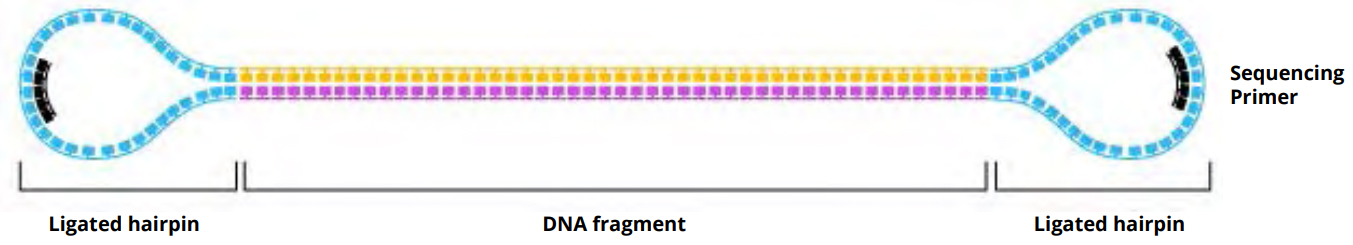
\includegraphics[width=\linewidth, height=0.05\textheight]{Pictures/Smrt_template.jpg}
		\caption{SMRT-bell template}\label{fig:smrtbell}
	\end{subfigure}
	\vspace{20pt}
	\hspace{5em}
	\begin{subfigure}{0.4\linewidth}
		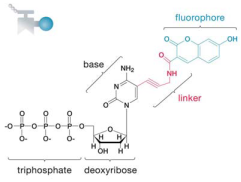
\includegraphics[width=\linewidth, height=0.2\textheight]{Pictures/Phospholinked_nucleotides.png}
		\caption{Phospholinked Nucleotides}\label{fig:Phospholinked_Nucleotides}
	\end{subfigure}
	\vspace{20pt}
	\begin{subfigure}{0.8\linewidth}
		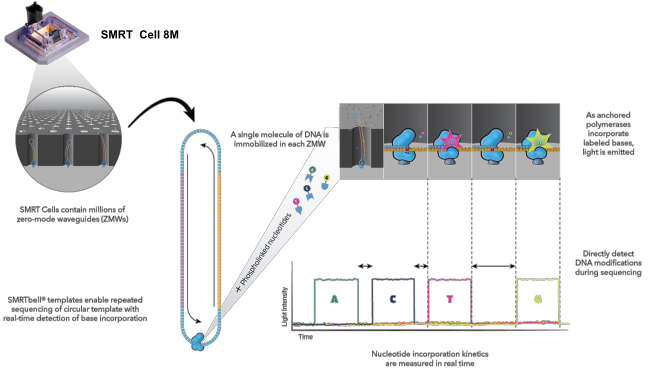
\includegraphics[width=\linewidth, height=0.3\textheight]{Pictures/Mechanism.png}
		\caption{PacBio Single-molecule real time sequencing}\label{fig:mechanism}
	\end{subfigure}
	\captionsetup{width=0.95\textwidth}
	\caption[PacBio SMRT]%
	{\textbf{PacBio SMRT}: At time of writing, PacBio released Sequel II with the provision of an 8M chip, containing 8 million wells, each capable of sequencing one single molecule. Figures adapted from PacBio}
	\label{fig:Mechanism}
\end{figure}

Currently, PacBio offers two sequencers: Sequel I and Sequel II; RSII was the first commercially available sequencer, but is no longer supported.

\subsubsection{Mechanism}
Due to the circular nature of the SMRT bell, the polymerase can continually read through the insert, and generate a continuous sequence of bases (continuous long read, CLR or polymerase read), which contains the hairpin adapter sequences. Pending on the polymerase lifetime and insert length, both strands can be sequenced multiple times, or “passes” in a CLR, which can then be delineated by the adapter sequences and resolved to multiple reads (subreads).  These subreads can be further collapsed to yield a highly-accurate Circular Consensus Sequence (CCS)(CCS\nomenclature{CCS}{Circular Consensus Sequence}). Further due to the circular nature of the SMRT bell, while sequencing and subsequent base-calling error can occur randomly at a rate of XXX, generating a raw accuracy of only 80\%, the generation of CCS from a coverage of 15 passes provides >99\% accuracy per base rate from sequence overlaps (Eid et al. 2009). The number of passes and subsequent generation of the CCS, however, is hindered by the length of the insert, whereby a long target DNA >XXX kB would only generate one single subread. 

\begin{figure}[h]
	\centering
	\vspace{20pt}
	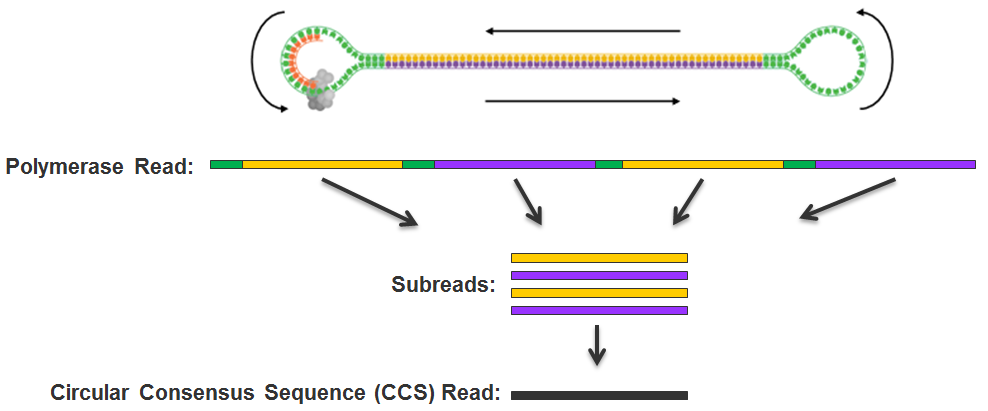
\includegraphics[width=0.8\linewidth, height=0.2\textheight]{Pictures/SMRTAdapter.png}
	\captionsetup{width=0.95\textwidth}
	\caption[Generation of Circular Consensus Sequence]%
	{\textbf{Generation of Circular Consensus Sequence}: CCS is generated by the collapse of multiple subreads, which sequence correspond to the double-stranded cDNA of interest. The greater the number of "passes" sequenced by the polymerase, the longer the polymerase read, the more subreads generated, and subsequently the higher the quality of CCS. Picture adapted from PacBio}
	\label{fig:CCS}
\end{figure}


\subsubsection{Performance and Run Quality Metric}
In an ideal situation, all the wells will contain an insert that will generate a positive signal. However, because XXXX, there will be some wells that are empty (quality metric denoted as P0: Productivity 0), and some wells that will be overloaded with multiple inserts with more than one polymerase (quality metric denoted as P2: Productivity: P2). Thus only wells that contain one polymerase (denoted as P1, Productivity 1) will generate a positive signal. Overloading may lead to increase in output of yield per SMRT cell, but increases the chance of P2 (multi-loaded ZMWs), resulting in shortened read lengths and lower accuracy compared to single-loaded ZMW. Loading can be optimised through titration.  	

A good run is defined by 50-70\% P1, a >XX kB polymerase read-length. Over-loading (>70\%) may result in reduced base quality (noisy base-calling), whereas under-loading (<50\%) results in lower throughput. A short polymerase read-length indicates sequencing/library preparation issues. These metrics are dependent on chemistry, pre-extension, and movie-runtime. 

\newpage
\section{Iso-Seq: Lab Pipeline}
In brief, the Iso-Seq protocol involved converting total RNA transcripts to full-length complementary DNA (cDNA) using the Clontech SMARTer PCR cDNA synthesis kit, which was then subsequently amplified and purified to generate double-stranded cDNA. The cDNA was then constructed to a SMRT bell library for sequencing. Size selection was not performed with full-length transcript detection of up to 4 kB. For targeted sequencing using IDT probes, all the steps in the Iso-Seq protocol are the same with an additional step of target capture post ds-DNA amplification and pre SMRT bell library. 

\subsection{CDNA synthesis}
\label{section:ch2_cDNA_synthesis_explanation} 
As part of the official Iso-Seq protocol, SMARTer PCR cDNA Synthesis Kit (Clontech) was used to convert extracted total RNA to complementary DNA by first strand cDNA synthesis, as outlined in Figure X. In brief, the polyA+ tails of RNA transcripts is first primed by a modified oligo (dT) primer, transcribed by SMARTScribe Reverse Transcriptase to generate a first single-stranded DNA, which is then diluted and subsequently amplified \cite{Ramskold2012}. All reagents were provided with the kit, except for the Pacific Bioscience’s barcodes, with all reagents and consumables used being sterile and DNAse and RNAse free. In order to sequence samples simultaneously (“multiplex”), as exploited for targeted sequencing, unique barcoded oligo (dT) primer was used in place of the standard oligo (dT) primer. With new Sequel system, cDNA can be sequenced without size selection. 

While this kit is advantageous in preferentially enriching for full-length cDNA sequences, as a template switching oligo is required to ensure complete reverse transcription, it cannot differentiate between intact and truncated RNA; which, present in poor-quality samples will be amplified as a potential source of contamination in the final cDNA library. One alternative is to exploit the 5’-cap that is present only in intact RNA and not truncated RNA (5-cap refers to the addition of 7-methylguanosine to the 5’-end of mRNA during transcription, to protect nascent mRNA from degradation and assist in protein translation). Alternative reverse transcriptase have been explored that only converts 5’capped mRNAs to cDNA, however, these have been found to negatively affect read length on the ONT platform (Cartolano et al. 2016). An alternative method, Full-Length cDNA Amplification (Teloprime), relies on a double-stranded adapter that recognises and ligates to the 5’cap at the end of first strand synthesis (Section X, Chapter 2)(\cite{Cartolano2016}). 

For this thesis, 200ng of total RNA was used for each sample for consistency and to ease downstream analyses. 

\subsection{PCR optimisation and DNA Amplification}
To minimise PCR bias (under or over-amplification), which can result in under or over representation of the different cDNA library size, the optimal number of PCR cycles for amplification of first-strand synthesis products was determined (Figure X). As described in Section X (Chapter 2), 5uL PCR aliquots were collected every two cycles (cycle 10, 12, 14, 16, 18) and run on a 1.5\% Agarose gel electrophoresis. With 200ng total input of total RNA, cycles 14 – 15 were selected for large scale amplification across all the mouse samples to generate sufficient amount of double-stranded cDNA product for SMRTbell library construction (Figure X). 

\subsection{AMPure Bead Purification} 
Post large scale amplification, the resulting PCR product was divided into two fractions and purified with 0.4X and 1X AMPure PB beads (PacBio), as described in Section X (Chapter 2).  In brief, ds-DNA was bound to the beads in either 1:1 or 1:0.4 ratio, which were then isolated on a magnetic rack, and washed with 70\% ethanol. DNA purification with 0.4x AMPure beads allows for enrichment of longer DNA fragments to provide a more representative library given that shorter fragments diffuse quicker into ZMW and are more likely to be sequenced. The ability to enrich for longer fragments is due to the preferential binding of beads to more negatively-charged, and subsequently larger molecular weight DNA, and thus displacement of shorter fragments.  Quantification and size distribution of each fraction was then determined using Qubit DNA High sensitivity assay (Invitrogen) and Bioanalyzer 2100 (Agilent), as described in Section X, Chapter X. Two fractions per sample were then recombined at equimolar quantities and library preparation performed using SMRTbell Template Prep Kit v1.0 (PacBio) (Figure X). 

The molarity was calculated by the following equation: 
\begin{equation}
\frac{concentration(\frac{ng}{ul})\times 10^6}{660(\frac{g}{mol}) \times average\:library\:size\:in\:bp\mbox{*}} = concentration\;in\; nM
\end{equation}
* the average library size was determined by the start and end point of the smear

\subsection{Target Capture using IDT Probes} 
As an additional step to the standard protocol for whole transcriptome sequencing for the targeted approach, amplified and purified cDNA was further enriched using IDT probes (Section X).  In brief, probes and blocking oligonucleotides were first added to cDNA, to allow hybridisation of probes to the target sequences/genes and oligonucleotides to the poly-T tract and cDNA primer to reduce non-specific binding. The hybridised library fragments were then incubated with washed magnetic streptavidin beads, and amplified using Takara Hot-Start polymerase (rather than KAPA HiFi from the official IDT protocol). The amplified library, still containing streptavidin beads, then underwent AMPure bead purification (Section X) for the elution of target cDNA (Figure X). SMRT Bell template preparation, primer and polymerase annealing was then proceeded. 

*Modifications to the protocol: waiting times at room temperature during hybridisation, lid heat temperatures, method of washing beads at room temperature; all modifications are incorporated from official IDT protocol, post amplification clean-up for consistency  

Targeted Sequencing

One current limitation of whole transcriptome sequencing is the low coverage/sequencing depth achieved per gene due to the distribution of reads across the whole transcriptome. Consequently, while whole transcriptome sequencing allows identification of novel genes (genes not previously annotated to the genome), it may not detect isoforms particularly those of low expression resulting in many false negatives. This can be circumvented by the use of target capture, which enriches a selective panel of genes that are then only sequenced. Multiple samples can further be pooled and sequenced together by barcoding samples at cDNA synthesis, which simplifies laboratory workflow and minimises associated sequencing costs.

[Other methods of Targeted Sequencing i.e. CRISPR]

Target genes is enriched from dsDNA using complementary IDT xGen Lockdown probes, which are individually synthesised, 5’ biotinylated DNA oligonucleotides. The hybrid capture is carried out using IDT xGEN hybridisation and wash kit protocol, using streptavidin-coated magnetic beads to bind and extract biotinylated probe-hybridised target DNA. 

120nt-long probes were designed to a panel of 20 AD-associated genes: Bin1, Trem2, Cd33, Vgf, FynMapt, Trpa1, Picalm, Sorl1, Abca7, Snca, Apoe, Abca1, App, Ank1, Clu, Fus, Ptk2b, Rhbdf2, Tardbp.  Two separate pools of the equal molar probes were created using the mouse genome (GRCm28/mm10) and human genome (GRCh37/hg19). To ensure full coverage of all transcripts, a list of probes was manually curated on the following criteria (Figure X): 
•	Ensured each exon in every gene is covered at least once (exons > 500bp has >1 probe) 
•	Removed any probes to intronic regions
•	Within each exon, removed any contiguous probes (as seen in the 1x tiling density) and ensured probes spaced 300-500bp (equivalent to 0.2x – 0.3x tiling density) 
•	From the contiguous “cluster”, selected probes with the highest GC content (40-65\% GC content)/minimal number of blast hits 
A full list of the number of probes per gene can be found in Supplementary X. The probes for all the target genes were delivered and resuspended in one pooled tube, in equimolar amounts. Note: no spike-in was added as control i.e. extra probe 


\subsection{SMRT Bell Template Preparation}
As described in Section X (Chapter 2), DNA Damage and End Repair was performed on the pooled library to polish ends of fragments for ligation of blunt hairpin adapters, necessary to generate high quality library of closed, circular SMRTBell templates. Any abasic sites were filled-in, thymine dimers resolved, and deaminated cytosine are alkylated. 3’ overhangs were removed, whereas 5’ overhangs were filled-in by T4 DNA Polymerase and phosphorylated by T4 PNK. Following 1x AMPure purification of repaired dsDNA, hairpin adapters were then ligated to the blunt ends for up to 24hours. Any fragments failed to ligate were removed with exonuclease III and VII. The repaired, ligated SMRT bell library was then purified twice with 1x AMPure beads, and assessed with Qubit DNA High sensitivity assay (Invitrogen) and Bioanalyzer 2100 (Analyzer) before proceeding to primer annealing and polymerase binding (Figure X). 

\subsection{Primer Annealing and Polymerase Binding} 
Post ligation of hairpin adapters, sequencing primer and polymerase were bound to both ends of the SMRTbell templates. The primer and polymerase to template ratio was critical to minimise under or –over loading, thus the concentration was sample specific. 

Prior to XXX chemistry, MagBead Loading was only recommended for IsoSeq SMRTbell libraries, whereas Diffusion Loading was recommended for all other applications with insert sizes from 
250 – 100001bp. As in the name, Diffusion Loading involves immobilization of polymerase-bound SMRTbells to ZMW by diffusion, whereas Magbead Loading involves immobilization by attachment to paramagnetic beads.  Diffusion loading thus preferentially loads longer transcripts, whereas magbead loading preferentially loads shorter transcripts of 700bp as it rolls across nanowells. 